\section{Data, samples, and detector}
\label{sec:data_detector}

We use DR10 cutouts to measure injection recovery and feature-space
differences between the observed and simulated samples.

\subsection{DESI Legacy Imaging Surveys DR10}
\label{sec:dr10_data}

We use $g$-, $r$-, and $z$-band coadded imaging from the tenth data release
(DR10) of the DESI Legacy Imaging Surveys \citep{Dey2019}.\footnote{DR10
description: \url{https://www.legacysurvey.org/dr10/description/}, accessed
29 August 2026.} The images have a
pixel scale of $0.262\;\mathrm{arcsec\;pixel^{-1}}$, and the nominal
$5\sigma$ point-source depths of the Legacy Surveys are $g \approx 24.7$,
$r \approx 23.9$, and $z \approx 23.0$~mag (AB). Because the delivered
point-spread function (PSF) and depth vary across the footprint and affect the
detectability of lensed features, these nominal depths characterise the survey
design rather than every location in DR10. Where these quantities enter the
injection experiments, we therefore use the local catalogue measurements at
each injection-target position rather than assigning one survey-wide value.

The Tractor catalogue is the model-based source catalogue produced from the
Legacy Surveys imaging \citep{Lang2016,Dey2019}.\footnote{DR10 catalogue
documentation: \url{https://www.legacysurvey.org/dr10/catalogs/}, accessed
29 August 2026.} For each catalogue object used in this
study, we extract a $101 \times 101$ pixel cutout
($26.5 \times 26.5\;\mathrm{arcsec}^{2}$) centred on its Tractor position.
Cutouts are stored in nanomaggies, for which the AB zeropoint is 22.5, and the
$g$, $r$, and $z$ images form the three detector input channels; no other DR10
catalogue or imaging products are used as detector inputs in this analysis.

\subsection{Preprocessing}
\label{sec:preprocessing}

We apply the same preprocessing to observed and injected cutouts. For each
band $b$, let $A$ denote the annulus containing pixels whose radial distance
from the cutout centre satisfies $20 \leq r < 32$ pixels. We define
\begin{equation}
 m_b = \operatorname{median}_{i \in A}(x_{b,i}), \qquad
 s_b = \operatorname{median}_{i \in A}\lvert x_{b,i}-m_b\rvert + 10^{-8},
\end{equation}
and transform each pixel as
\begin{equation}
 x'_{b,i} =
 \operatorname{clip}\left(\frac{x_{b,i}-m_b}{s_b},-10,+10\right).
\label{eq:raw_robust}
\end{equation}
Thus, each band is centred and scaled using a robust local reference while
preserving the full $101 \times 101$ field. The scale \(s_b\) is the unscaled
median absolute deviation (MAD), rather than a Gaussian-equivalent standard
deviation.

All detector comparisons retain the $20$--$32$ pixel normalisation annulus
used during training. The annulus can contain light from the central object or
injected source, so its median and MAD can depend on astrophysical structure
as well as the local background. These statistics define the detector's
trained input mapping.

\subsection{Detector development and evaluation roles}
\label{sec:data_roles_overview}

Table~\ref{tab:detector_roles_overview} summarizes the samples used for
training, validation, threshold calibration, and evaluation. Development
positives are noisy labels from the literature-reviewed candidate set and the
lower-confidence catalogue-candidate set; confirmed lenses are reserved for
evaluation. False-positive rate (FPR) denotes the fraction of catalogue-negative
examples at or above threshold. We calibrate the threshold
on one negative sample and estimate its FPR on another.

\begin{table*}
\caption{Detector-development and evaluation roles. ``Reviewed candidates''
are Lenscat systems classified as candidates---rather than confirmed lenses,
non-lenses, or uncertain systems---after object-level review of the published
evidence.
``Additional catalogue candidates'' are lower-confidence catalogue records
used only as noisy positive examples. The calibration, achieved-FPR, and
selected-system samples are disjoint and are used only after training.}
\label{tab:detector_roles_overview}
\centering
{\small
\setlength{\tabcolsep}{4pt}
\begin{tabular}{L{0.21\textwidth}rL{0.29\textwidth}L{0.27\textwidth}}
\toprule
Role & Negative examples & Positive or observed examples & Function \\
\midrule
Training: reviewed + additional &
286\,679 & 238 reviewed candidates + 3\,395 additional catalogue candidates &
Primary training set; 290\,312 rows \\
Validation: reviewed + additional &
61\,437 & 64 reviewed candidates + 714 additional catalogue candidates &
Development diagnostics and sensitivity-checkpoint selection; 62\,215 rows \\
Training: reviewed candidates only &
286\,679 & 238 reviewed candidates &
Alternative positive-label composition; 286\,917 rows \\
Validation: reviewed candidates only &
61\,437 & 64 reviewed candidates &
Checkpoint selection for the corresponding runs; 61\,501 rows \\
Full test partition &
61\,435 & 63 confirmed systems &
Source partition for final evaluation roles \\
Threshold calibration &
20\,002 & None &
Set the primary or checkpoint-specific operating threshold \\
Achieved-FPR evaluation &
12\,512 & None &
Evaluate catalogue-negative threshold exceedance \\
Selected-system evaluation &
None & 43 confirmed systems &
Recovery among the 43 selected confirmed systems \\
Exploratory-analysis-development role &
None & 20 confirmed systems &
Excluded from endpoint and observed-reference denominators \\
\bottomrule
\end{tabular}
}
\end{table*}

\subsection{Labelled samples and provenance}
\label{sec:sample_provenance}

Lenscat v1.1.3 is the public, community-contributed strong-lens catalogue
compiled by \citet{Vujeva2025} and archived by \citet{LenscatV113}.

The positive parent catalogue was assembled from Lenscat. We selected
5,104 entries whose names identified them with DESI imaging; 4,788 were
associated with a Tractor source in the processed DR10 sweeps within
5~arcsec. Lenscat places 389 of these systems in its highest-confidence
category and 4,399 in a lower-confidence candidate category. All 389
highest-confidence records underwent object-level literature review. The
4,399 lower-confidence records supplied noisy positive labels for detector
development, subject to the role exclusions in
Section~\ref{sec:training_sets}. Lenscat
confidence was not treated as confirmation because its highest category can
denote either spectroscopically confirmed multiple images or the highest grade
assigned by a contributing study \citep{Vujeva2025}. The entries originate from heterogeneous
discovery samples, including the DESI Legacy Imaging Surveys searches of
\citet{Huang2020,Huang2021}, \citet{Stein2022}, and \citet{Storfer2024}.

Literature review identified 63 confirmed lenses among the 389 reviewed
systems. Of these, 50 have secure spectroscopic redshifts for both deflector
and source, seven have secure lens evidence but incomplete or
lower-confidence spectroscopy, and six are confirmed by imaging or lens
modelling without secure redshifts for both components. The available
literature provides heterogeneous spectroscopic and imaging support across
the cohort. The four non-lenses and two uncertain systems are excluded from
lens-performance estimates; the remaining 320 candidates form the reviewed
source of noisy positive labels for detector development. For the 43-system
evaluation cohort, object-level confirmation evidence and available
deflector and source redshifts are listed in Appendix
Table~\ref{tab:confirmed_43_provenance}.

\begin{table}
\caption{Literature-based classifications for the 389 reviewed Lenscat
records.}
\label{tab:evidence_review_status}
\centering
\begin{tabular}{lr}
\toprule
Scientific status & Number \\
\midrule
Confirmed lens & 63 \\
Candidate & 320 \\
Confirmed non-lens & 4 \\
Uncertain & 2 \\
\midrule
Total & 389 \\
\bottomrule
\end{tabular}
\end{table}

The negative parent sample was drawn from the Tractor catalogue in two stages.
The sampling frame required finite coordinates,
$-18^\circ < \delta < +32^\circ$, a Tractor morphological type of SER, DEV,
or REX, at least three exposures in each of \(g,r,z\), and none of mask bits
1, 5, 6, 7, 11, 12, or 13. It also required a separation of at least
11~arcsec from the 5,104-entry DESI-named Lenscat parent catalogue. For rows
with positive fitted \(z\)-band flux, the observed magnitude, not corrected
for Galactic foreground extinction, had to satisfy \(z<20\). Rows with
finite non-positive \(z\)-band flux have no logarithmic magnitude and were
therefore retained without the \(z<20\) requirement; the available records do
not document a scientific reason for this exemption. Colour was not an
eligibility cut, but \(g-r\) contributed to the sampling strata described
below. All reported analyses use this fixed sample. The available sampled-row
table retains the \(z\)-band exposure count but omits the corresponding
\(g\)- and \(r\) columns. The archived roster and image cutouts are sufficient
to reproduce the reported analyses, but the available table does not contain
the \(g\)- and \(r\)-band exposure counts needed to recheck those two
eligibility criteria row by row.

Rows in the sampling frame were assigned to two sampling strata. \(N1\)
contains the remaining candidates; \(N2\) uses proxies for lens-like negative
morphology and is assigned by the first matching condition: DEV type with
\(r\)-band flux at least 5~nmgy; SER or DEV type
with Tractor \(\mathtt{shape\_r}\geq1.8\)~arcsec;
\(g-r\leq0.4\) and \(r\leq20.5\)~mag; or
\(\mathtt{shape\_r}\geq2.0\)~arcsec and \(r\)-band flux at least 3~nmgy.
These proxies stratify sampling; they are not eligibility cuts and do not use
detector scores. Within exposure-count and Tractor-type strata, the procedure
targeted an 85:15 \(N1:N2\) sample before final eligibility filtering.

The sampler drew 453,100 rows. Of these, 6,207 lacked a final cutout, leaving
446,893 rows with usable pixels. The final negative pool additionally
required finite \(g,r,z\) photometry and removed any row within 11~arcsec of a
Lenscat system or catalogue-positive centre. A total of 37,342 usable-cutout
rows failed at least one of these final photometry or proximity rules.
The retained pool therefore contains 409,551 catalogue-negative rows:
343,469 in \(N1\) and 66,082 in \(N2\). The final stratum proportions need not
equal the sampling target because eligibility was applied after sampling.
These are catalogue negatives, not individually verified non-lenses.

The positive and negative parent samples were not selected under identical
eligibility rules. In particular, the magnitude, morphology, exposure, mask,
and declination restrictions above were not applied to the positive
catalogue. Eight of the 63 confirmed lenses, and 2,291 of all 4,788
catalogue-positive rows, lie outside the negative sample's declination
window. The observed--injected comparison therefore includes differences in
deflector populations and survey conditions alongside source insertion.

\subsection{Development and test partitions}
\label{sec:data_partitions}

The clean sample contains 409,551 negatives and 63 confirmed lenses. Before
noisy candidate labels are added, the grouped split assigns 286,679 negatives
to training, 61,437 to validation, and 61,435 to test; all 63 confirmed lenses
are assigned to test before model development. No noisy candidate label is
counted as confirmed.

Rows were grouped by object identity, sky proximity, overlapping cutouts,
NSIDE$=128$ NESTED HEALPix cell \citep{Gorski2005}, and known physical system
before partitioning. These grouping rules keep objects linked by the recorded
identities and spatial or physical-system information within the same
partition. Candidate labels were added under the same grouping rules.

Before detector scoring, disjoint spatial groups supplied 20,002 negatives
for threshold calibration and 12,512 for false-positive-rate evaluation. The
63 confirmed systems were excluded from detector fitting, validation,
checkpoint selection, and threshold calibration. Twenty had an exploratory
feature-analysis-development role and are excluded from all final endpoint and
observed-reference denominators. The published roster of the remaining 43
systems defines the selected-system endpoint and the observed-reference
sample. We do not have a documented general scientific eligibility rule that
independently selects those 43 from all 63 confirmed systems. The 43-system
roster was not chosen using detector scores.
No development object shares a recorded identity or physical group with the
calibration, evaluation, or injection samples. Where a spatial-component
identifier is available, it also shows no shared component; the calibration,
achieved-FPR, and injection-target samples additionally have no flagged
development HEALPix or 38-arcsec contact. The available identities, group
labels, and sky-neighbour checks show no recorded overlap between development
and evaluation samples. Exact footprint polygons are unavailable for part of
the development set, so broader geometric overlap cannot be tested. The
selected-system recovery fraction is a finite-cohort summary of these 43
heterogeneous systems.

\subsection{Positive examples and training-set composition}
\label{sec:training_sets}

Because the clean training and validation partitions contain no confirmed
positive examples, detector training uses noisy catalogue-positive labels.
The 320 objects assigned candidate status after literature review provide one
source of positive examples; the 4,399 lower-confidence catalogue candidates
provide an additional source. Rows spatially linked to the test partition are
excluded before the development sets are formed. This removes 18 reviewed
candidates and 290 additional catalogue candidates.

The primary training set combines reviewed and additional catalogue candidates;
the comparison set uses reviewed candidates only, with the same negatives
(Table~\ref{tab:detector_roles_overview}). Their training negative-to-positive
ratios are approximately \(79{:}1\) and \(1205{:}1\), respectively. Confirmed
lenses, confirmed non-lenses, and uncertain systems enter neither composition.

Both positive-example sets contain candidate labels rather than uniform
confirmed truth; the contamination fraction of the additional catalogue
candidates has not been measured.
In natural-prevalence runs, training rows are shuffled and sampled without
replacement each epoch, with the incomplete final mini-batch omitted; the
loss is unweighted binary cross-entropy. Accuracy is not used for checkpoint
selection or operating point assessment because an all-negative classifier
would be favoured by the class imbalance while recovering no labelled
positives.

\subsection{Primary detector protocol}
\label{sec:detector_training}

The finder is an ImageNet-initialised EfficientNetV2-S with a binary output
\citep{Deng2009,Russakovsky2015,TanLe2021}, subsequently trained for lens
classification. ImageNet-1K is a labelled natural-image dataset whose pretrained
weights supply a general visual initialization. The trained finder's pooled
representation and the distinct external feature protocols are defined in
Section~\ref{sec:linear_probe_methods}.

The primary run uses reviewed and additional catalogue candidates, seed 42,
natural-prevalence sampling, and a cosine learning-rate schedule. It trains
for 160 epochs with AdamW, a five-epoch learning-rate warm-up, and the
backbone frozen for the first five epochs. The initial learning rate is
\(3.88\times10^{-4}\), and weight decay is \(10^{-4}\). Training uses
mixed-precision forward passes, micro-batches of 64 accumulated to an
effective batch size of 512, and omits the incomplete final mini-batch. Early
stopping is disabled.
Horizontal and vertical flips are applied independently with probability 0.5,
followed by a rotation selected uniformly from $0^\circ$, $90^\circ$,
$180^\circ$, and $270^\circ$. We use no colour or noise augmentation.

The primary detector is the epoch-160 checkpoint; validation, calibration,
and evaluation scores do not select it. All primary-detector evaluations use the same
preprocessing and operating threshold defined in
Section~\ref{sec:scoring_contract}.

\subsection{Detector-sensitivity training panel}
\label{sec:checkpoint_panel_design}

The sensitivity panel contains 12 EfficientNetV2-S runs that share the
primary architecture and training duration but vary the positive sample,
random seed, sampler, or learning-rate schedule:
\begin{itemize}
\item six baseline runs cross the two positive-example sets---reviewed
candidates only, or reviewed plus additional catalogue candidates---with
seeds 42, 123, and 2026 under natural-prevalence sampling and cosine
scheduling;
\item two sampler runs use seed 42 and seeded 50:50 class-balanced
weighted sampling with replacement for the two positive-example sets;
\item two schedule runs use seed 42 and natural-prevalence sampling for the
two positive-example sets, with a step schedule that halves the learning rate after epoch
130 instead of cosine decay; and
\item two additional runs use reviewed candidates only, with seeds 7 and 2027
under the baseline sampler and schedule.
\end{itemize}
The repeated seeds probe sensitivity to training stochasticity; they are not a
statistical sample of all possible trained models. Sampler and schedule pairs
change one training choice at seed 42. Changing the positive sample also
changes its composition, prevalence, and size; that comparison measures
detector sensitivity to the combined change.

For each sensitivity run, we select the checkpoint with the highest validation
average precision; selected epochs range from 17 to 103. These checkpoints
form a secondary analysis; the epoch-160 checkpoint remains the primary
detector.
Appendix~\ref{app:checkpoint_sensitivity} reports the complete panel.

Figure~\ref{fig:data_training_flow} summarizes the sample, training, and
evaluation roles.

\begin{figure*}
\centering
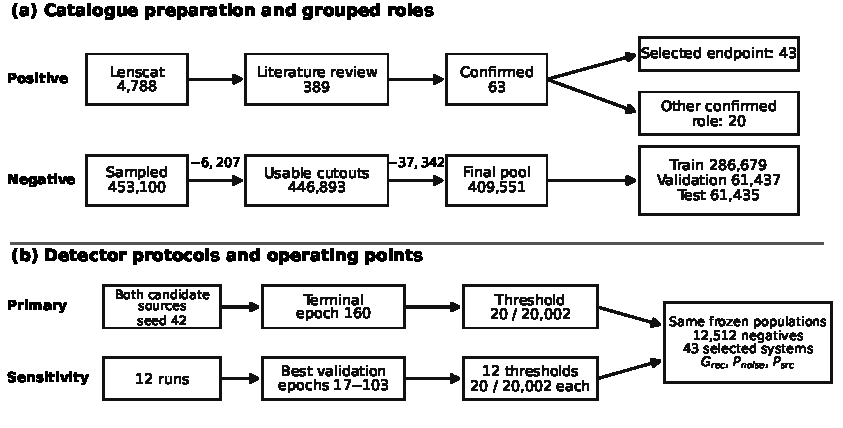
\includegraphics[width=\textwidth]{figures/section2_data_training_flow.pdf}
\caption{Data preparation, detector training, and evaluation roles. Panel A
shows the catalogue-positive evidence review and the negative-sample flow
before grouped train, validation, and test assignment. Panel B separates the
primary terminal-epoch protocol from the 12-run validation-selected
sensitivity panel. The primary detector and each sensitivity checkpoint use
the same 20,002-row calibration population. Each model is calibrated
independently by choosing the threshold with 20 exceedances, then evaluated
on the same corresponding held-out cohorts. The primary uses reviewed and
additional catalogue candidates. The sensitivity panel includes both
positive-sample compositions and the specified sampler, schedule and seed
variants. Arrows show data or model flow; evaluation does not feed back into
training.}
\label{fig:data_training_flow}
\par\smallskip{\raggedright\noindent\textit{Alt text:} Two linked flow diagrams. The first
tracks catalogue positives to 63 confirmed systems and tracks 453,100 sampled
negatives to 409,551 retained rows and grouped data partitions. The second
shows noisy-label training sets feeding the primary epoch-160 detector and a
12-run sensitivity panel, followed by separate calibration thresholds and
the same held-out evaluation samples.\par}
\end{figure*}
